\chapter{绪论}\label{chap:introduction}{
  \section{本文研究背景与意义}
  随着信息技术迅猛发展,计算密集型任务与数据密集型任务已成为人工智能、流媒体、大数据、云计算和科学计算等领域面临的双重挑战。
  在这种要求下,大规模分布式集群系统被提出,要求应用多重并行编程模型,结合松耦合任务调度与数据共享策略,实现跨节点的负载均衡与任务协作。

  从并行编程的角度来看,这些范式基于以下并行模型:共享内存、消息传递和分
  布式共享内存。这三种模型在编程时分别具有如下特点:
  \begin{itemize}
    \item \textbf{共享内存模型}: 所有计算核心共享一块全局主存,并通过各自私有的高速缓存(cache)来存储数据副本以加速数据访问;
    \item \textbf{消息传递模型}: 消息传递模型赋予集群中各节点上的进程独立的虚拟地址空间,进程间通过显式的通信原语(如 Send/Recv)完成数据交换;
    \item \textbf{分布式共享内存模型}: 相当于共享内存模型在分布式系统上的扩展,将共享的理念从片上、节点内扩展到集群中,在物理上分离的内存之上构建一个虚拟共享内存抽象层,底层通过消息传递实现特定的迁移机制以完成数据共享。
  \end{itemize}

  上述三种模型中,分布式共享内存(Distributed Shared Memory, DSM)结合了共享内存与消息传递的优势,展现出以下核心特征:
  \begin{enumerate}[leftmargin=1em, align=left]
    \item \textbf{相较于消息传递:} 其采用透明的数据共享机制并保持与传统共享内存编程模型一致的抽象层,显著降低了分布式应用开发的复杂度;
    \item \textbf{相较于多核共享内存架构:} DSM 通过分布式扩展突破了单节点内存容量限制,在构建大规模负载处理系统时展现出更优的性价比;
  \end{enumerate}

  然而,DSM 仍面临两个关键挑战:昂贵的跨节点通信时延开销以及分布式环境下数据一致性维护的复杂性代价。

  长期以来,由于这两个挑战以及单节点内多核处理器所展现的强大计算能力,分布式共享内存系统在大规模集群中的应用受到较大限制。
  但随着高性能网络互连和远程内存访问(RDMA)技术的不断进步,为解决传统消息传递模型中显式数据分区和通信管理的复杂性提供了全新思路。
  当今的分布式共享内存系统不仅有助于突破单节点内存容量的局限,还能在保证数据一致性的前提下,支持更大规模、更高并发的数据处理任务。

  % \begin{figure}[!htbp]
  %   \centering
  %   \begin{subfigure}[b]{0.35\textwidth}
  %     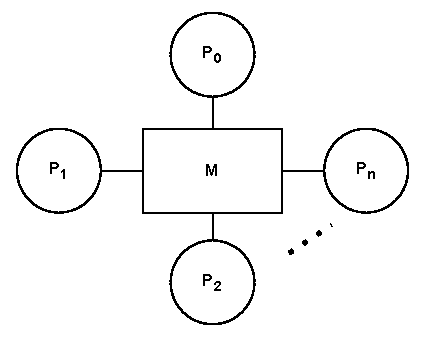
\includegraphics[width=\textwidth]{Img/共享内存模型.drawio.pdf}
  %     \caption{共享内存模型}
  %     \label{fig:multi-core}
  %   \end{subfigure}%
  %   \hspace{1.5cm}
  %   \begin{subfigure}[b]{0.35\textwidth}
  %     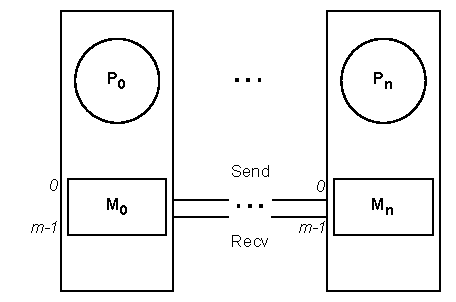
\includegraphics[width=\textwidth]{Img/消息传递模型.drawio.pdf}
  %     \caption{消息传递模型}
  %     \label{fig:message-passing}
  %   \end{subfigure}
  %   \begin{subfigure}[b]{0.6\textwidth}
  %     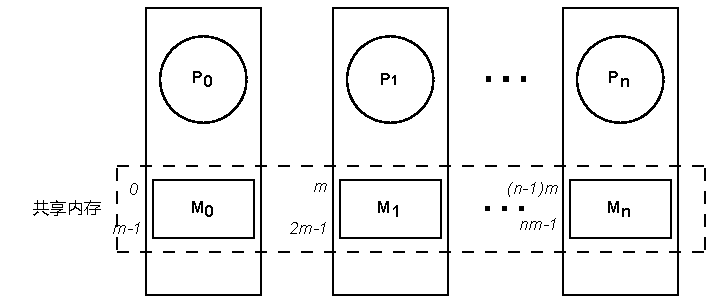
\includegraphics[width=\textwidth]{Img/分布式共享内存模型.drawio.pdf}
  %     \caption{分布式共享内存模型}
  %     \label{fig:dsm}
  %   \end{subfigure}
  %   \bicaption{并行编程模型}{Parallel programming model}
  %   \label{fig:model}
  % \end{figure}

  本文基于国产软件分布式共享内存系统 JIAJIA\citep{huweiwu2001sma,huweiwu2024ca,1999huweiwuJIAJIA} 进行研究。
  JIAJIA 由胡伟武老师于 90 年代末设计,是我国首款自主研发的 SDSM 系统。
  其采用页粒度共享,并基于 NUMA 架构构建虚拟共享内存,通过缓存机制加速远程访问,节点之间采用单线程 UDP 通信进行数据交换。
  JIAJIA 的问世填补了国内研究空白,并被全球 100 余家科研机构采用,成功应用于国产高性能计算机。

  在此基础上,M-JIAJIA进行了以下两个方面的优化:
  \begin{enumerate}
    \item M-JIAJIA 设计并实现了同时支持 UDP 和 RDMA 的双通信栈,不仅有效缓解了传统软件 DSM 系统的网络瓶颈,
          也为高性能网络环境下的软件分布式共享内存系统提供了探索方向;
    \item M-JIAJIA 通过将通信流程拆分为入队、发送、监听、接收和处理五个阶段,并利用多线程机制构建流水化通信模型,实现并行加速,
          从而充分利用底层硬件资源。
  \end{enumerate}

  在系统设计与实现过程中,M-JIAJIA 始终围绕可靠性、可扩展性与易用性的平衡,遵循以下核心设计原则:
  \begin{itemize}
    \item 正确性的优先级始终高于性能优化;
    \item 系统设计层次化、核心逻辑模块化,便于后续维护和扩展;
    \item 在不损害性能的前提下,尽可能增加系统易用性和灵活性。
  \end{itemize}

  % \subsection{软件分布式共享内存系统概述}
  % 根据节点间内存访问的耦合程序、一致性协议实现层级以及典型应用场景,分布式共享内存系统可以分为紧耦合(Tightly-Coupled)与松耦合(Loosely-Coupled)两类。
  % \begin{itemize}
  %   \item 紧耦合分布式共享内存系统以硬件为核心实现全局内存地址空间抽象,通常依赖于专用互连架构(如ccNUMA,NUCA)与定制缓存一致性协议(如MESI/MOESI);
  %   \item 松耦合分布式共享内存系统则是指在物理分散节点间构建逻辑统一的共享内存抽象的软件或轻量级硬件辅助实现(如表~\ref{tab:dsm-different-implementations}所示)。
  % \end{itemize}

  % \begin{table}[!htbp]
  %   \bicaption{DSM的不同实现级别}{Different levels of DSM Implementation}% caption
  %   \label{tab:dsm-different-implementations}
  %   \centering
  %   \footnotesize% fontsize
  %   \setlength{\tabcolsep}{4pt}% column separation
  %   \renewcommand{\arraystretch}{1.5}% row space 
  %   \begin{tabular}{lcc}
  %     \hline
  %     DSM 实现级别 & 要求               & 示例                            \\
  %     \hline
  %     硬件       & 专用硬件(共享缓存、片上互连等) & ccNUMA、NUCA                   \\
  %     系统软件     & 操作系统虚拟管理机制修改     & IVY、Munin等                    \\
  %     运行时用户库   & 基础通信能力           & TreadMarks、JIAJIA、OpenSHMEM 等 \\
  %     语言或语言扩展  & 编译器支持            & PGAS语言(UPC、UPC++),OpenMP等     \\
  %     \hline
  %   \end{tabular}

  %   \vspace*{3ex}

  %   \begin{minipage}{\textwidth}% choose width suitably
  %     \mdseries\par\setlength\hangindent{2\ccwd} 表注:这里并不是严格划分,一些 DSM 的实现可能涉及多个层级协同实现。
  %   \end{minipage}
  % \end{table}

  相比紧耦合分布式共享内存系统,属于松耦合范畴的软件 DSM 系统的实现较为灵活,
  可以在系统软件(操作系统或编译器)、运行时库、语言等多个层次实现,具体区分可参见~\ref{sec:implementations}小结内容。


  \subsection{软件分布式共享内存系统发展历程}
  \begin{enumerate}[leftmargin=1em, align=left]
    \item \textbf{早期DSM系统在内存一致性方面的发展历程}

          \begin{itemize}
            \item \textbf{顺序一致性}: 1986 年,Li Kai 博士在论文\citep{likai1986svm} 中验证了在分布式系统上构建共享虚拟内存(SVM)的可行性,并开发了首个软件 DSM 系统 IVY\citep{likai1988ivy}。
                  IVY 采用 页粒度共享,支持 SWMR 访问模式,通过 顺序一致性 保持数据一致性,在并行计算中取得良好加速效果。
            \item \textbf{释放一致性(急切更新)}: Munin\citep{bennett1990munin} 采用 释放一致性(RC),仅在特定同步点执行一致性操作,降低通信开销。
                  同时,它使用 数据类型特定一致性模型,结合 多写协议 与 延迟更新机制,有效缓解假共享问题。
            \item \textbf{释放一致性(懒惰更新)}: TreadMarks\citep{amza1996treadmarks} 提出 懒惰更新释放一致性(LRC),
                  相比 Munin 的急切更新,仅在锁的最后释放者和新获取者之间传播一致性消息,从而减少通信量。
            \item \textbf{域一致性}: JIAJIA\citep{huweiwu2001sma} 采用 域一致性(SC),比 LRC 更宽松,仅同步锁保护区域的修改。
                  其 基于锁的缓存一致性协议 用锁存储写通知,而非目录,减少管理复杂性,提升可扩展性。
          \end{itemize}

    \item \textbf{软件 DSM 研究热度下降}

          多核架构普及后,片内通信远快于 DSM 依赖的网络通信,使得软件 DSM 失去优势。
          研究方向逐渐转向 优化一致性协议 和 减少通信次数\citep{Cheung1999AMP, abe2003movinghomedsm}。
          \begin{itemize}
            \item 研究趋势:
                  \begin{itemize}
                    \item 一致性协议优化(减少通信开销)。
                    \item 减少数据传输量(如写通知、失效消息优化)。
                  \end{itemize}
          \end{itemize}

    \item \textbf{FaRM:RDMA 在 DSM 中的应用}

          2014 年,微软 FaRM\citep{drago2014farm} 首次结合 RDMA + DSM,替代 TCP/IP,显著降低通信延迟,提升吞吐量,引发后续研究。
          证明 RDMA + DSM 组合的可行性,推动 RDMA 在 DSM 研究中的应用。

    \item \textbf{RDMA 驱动的后续 DSM 研究}

          \begin{itemize}
            \item \textbf{DaRPC(2014)}:基于 RDMA 实现 异步非阻塞 RPC,减少通信延迟。
            \item \textbf{FaSST(2016)}:使用 RDMA Send/Recv 语义 提供高吞吐事务处理。
            \item \textbf{Argodsm(2015)}:提出 自失效(self-invalidation)+ 自降级(self-downgrade),减少一致性维护开销,使用 MPI 作为通信底层。
            \item \textbf{Grappa(2015)}:支持 数据密集型计算,利用多线程优化任务调度,但底层仍基于 MPI,而非 RDMA。
            \item \textbf{GAM(2018)}:采用 部分存储一致性(PSO),通过 RDMA Send/Recv + Write 进行数据传输,提高吞吐量。
            \item \textbf{Drust(2024)}:结合 Rust 所有权模型 限制读写顺序,降低一致性开销,与 SWMR 访问模式兼容。
          \end{itemize}

  \end{enumerate}

  \subsection{软件分布式共享内存系统的机遇与挑战}
  在新型硬件架构和应用场景变革的双重驱动下,现代软件分布式共享内存系统正迎来前所未有的机遇与挑战。

  \textbf{机遇:RDMA 高速网络。}RDMA 技术显著降低了跨节点访存开销,且持续优化,未来 RDMA 网络带宽有望达到 Tbps 级别。
  例如,英伟达 ConnectX-8 网卡带宽已达 800 Gbps,接近本地内存速度,甚至优于某些 NUMA 节点间通信通道(如 QPI)。
  这一趋势极大缓解了传统软件 DSM 系统的高延迟通信瓶颈。

  \textbf{挑战:强一致性与高性能之间的平衡。} 尽管高速网络降低了传输延迟,但在软件 DSM 系统中实现严格的内存一致性(如顺序一致性)仍会引入同步开销,制约系统性能。
  如何在一致性与高性能之间找到平衡,仍是当前软件 DSM 系统的关键挑战。

  \section{本文研究内容与主要贡献}
  本文对软件分布式共享内存系统为开发人员提供了一个传统的类似多线程编程的共享内存抽象,同时尽可能运用到当前的RDMA网络技术,来加速整个系统之间的通信速度。

  针对上述,本文的主要贡献有:
  \begin{enumerate}[leftmargin=1em, align=left]
    \item 设计并实现了一个支持双通信栈(UDP+RDMA)的软件分布式共享内存系统 M-JIAJIA,充分利用RDMA新型网络技术的高带宽;
    \item 采用多线程加速M-JIAJIA系统的通信速度,改变了JIAJIA传统的单线程信号驱动通信模型;
    \item 设计并实现系统取页时的远程预取机制,降低通信次数,大大提升了具有强局部性的应用程序的性能;
    \item 深入分析了基于 \texttt{M-JIAJIA} 库的应用程序在各阶段的性能开销,并对 M-JIAJIA 与 OpenMPI 的关键接口进行了对比测试,为后续相关研究提供了重要的参考与支撑。
  \end{enumerate}
  % 4. 利用 \texttt{M-JIAJIA} 设计实现了 \texttt{jacobi} 迭代算法,可用来在集群上进行线性方程组和热度扩散计算。
  \section{本文组织结构}
  第\ref{chap:introduction}章介绍了文章的研究背景和意义,回顾了软件 DSM 系统的发展历程以及现如今所面临的挑战与机遇,概述本文工作的研究内容和主要贡献;

  第\ref{chap:sdsm}章主要介绍工作所涉及的两个技术基础——软件分布式共享内存和RDMA,论述了软件 DSM 系统所涉及的关键技术以及软件 DSM 的系统设计,并介绍了 RDMA 技术的工作原理;

  第\ref{chap:JIAJIA}章主要介绍JIAJIA系统的相关设计,介绍了其基本的实现原理与一致性模型;

  第\ref{chap:MJIAJIA}章主要介绍了M-JIAJIA的具体设计与实现;

  第\ref{chap:RDMA}章具体介绍了M-JIAJIA 的 RDMA 通信栈的设计与实现;

  第\ref{chap:experiments}章主要介绍关于 M-JIAJIA 系统的性能分析与优化测试;

  第\ref{chap:summary}章对本文的工作进行了总结,并展望 M-JIAJIA 系统后续可能的应用和研究方向。
}
